\documentclass[12pt, titlepage]{report}
\usepackage{consumer_resource_final}
\graphicspath{{./figures/}}

\begin{document}
% \subsection{Time evolution}
% \begin{figure}[h!]
% \centering
% 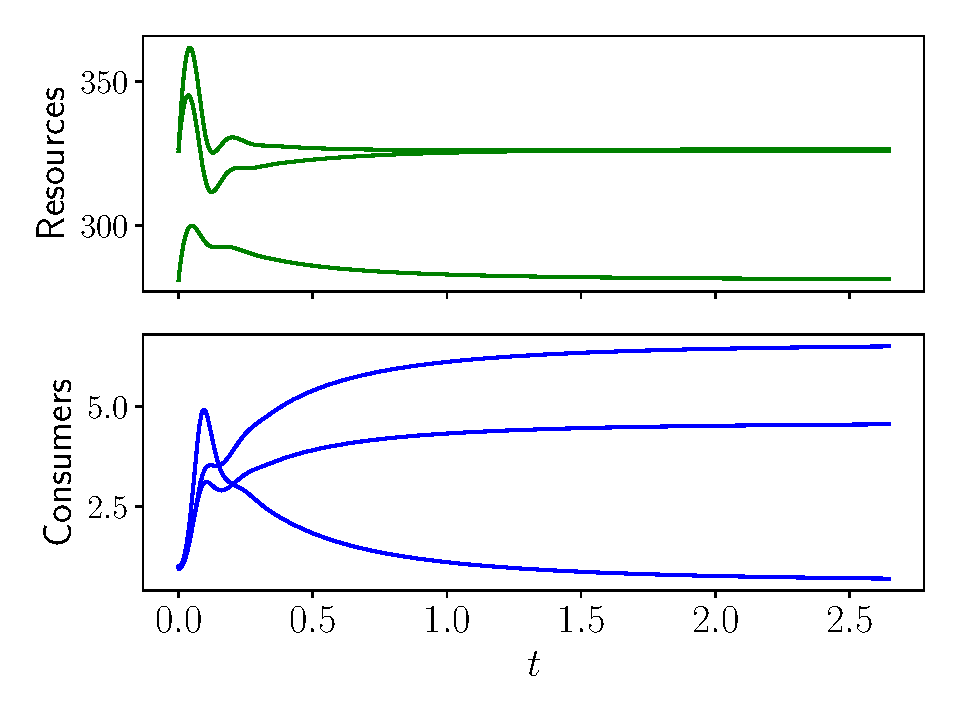
\includegraphics[width=0.6\linewidth]{Typical_time_evolution/Typical_time_evolution_resources_species_high_threshold.pdf}
% \caption{Time evolution for high coefficient threshold ($\epsilon_{\text{conv}}=10^{-1}$)}
% 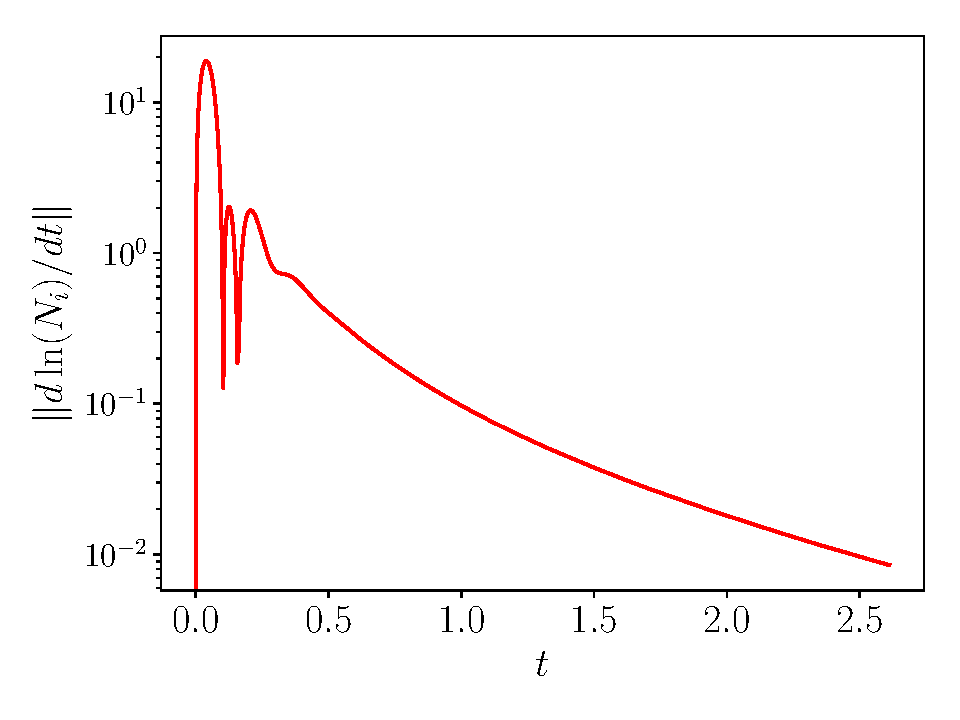
\includegraphics[width=0.6\linewidth]{figures/Typical_time_evolution/Typical_time_evolution_log_derivative_high_threshold.pdf}
% \caption{Typical convergence to judge equilibrium, we see the simulation stops at $\epsilon_{\text{conv}}=10^{-1}$}
% \end{figure}
% \begin{figure}[h!]
% \centering
% 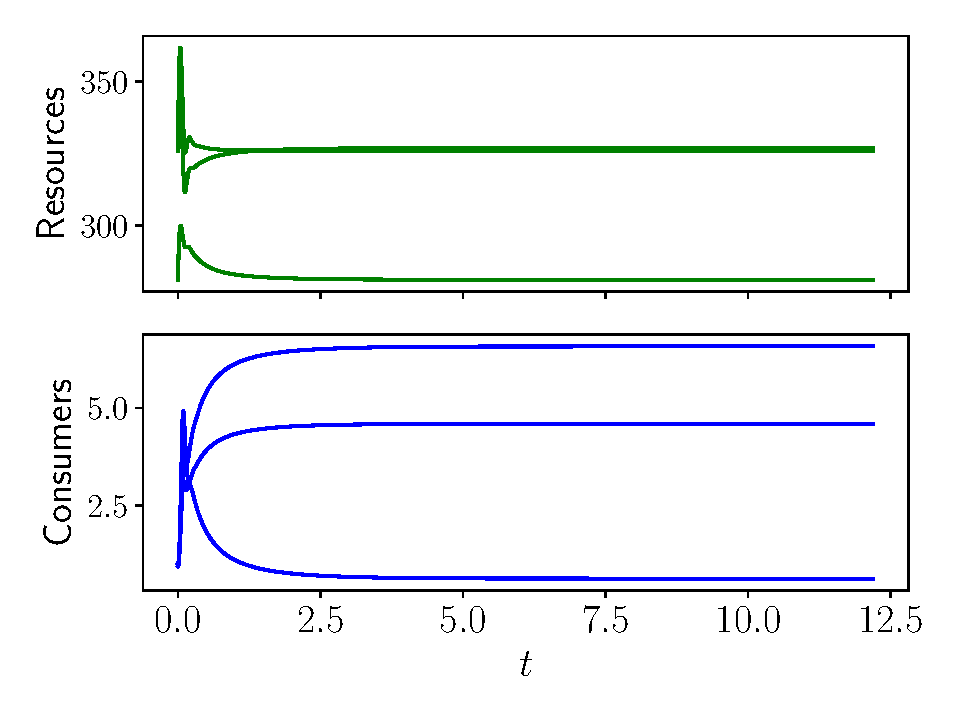
\includegraphics[width=0.6\linewidth]{Typical_time_evolution/Typical_time_evolution_resources_species_low_threshold.pdf}
% \caption{Time evolution for low coefficient threshold (more accuracy) ($\epsilon_{\text{conv}}=10^{-5}$)}
% 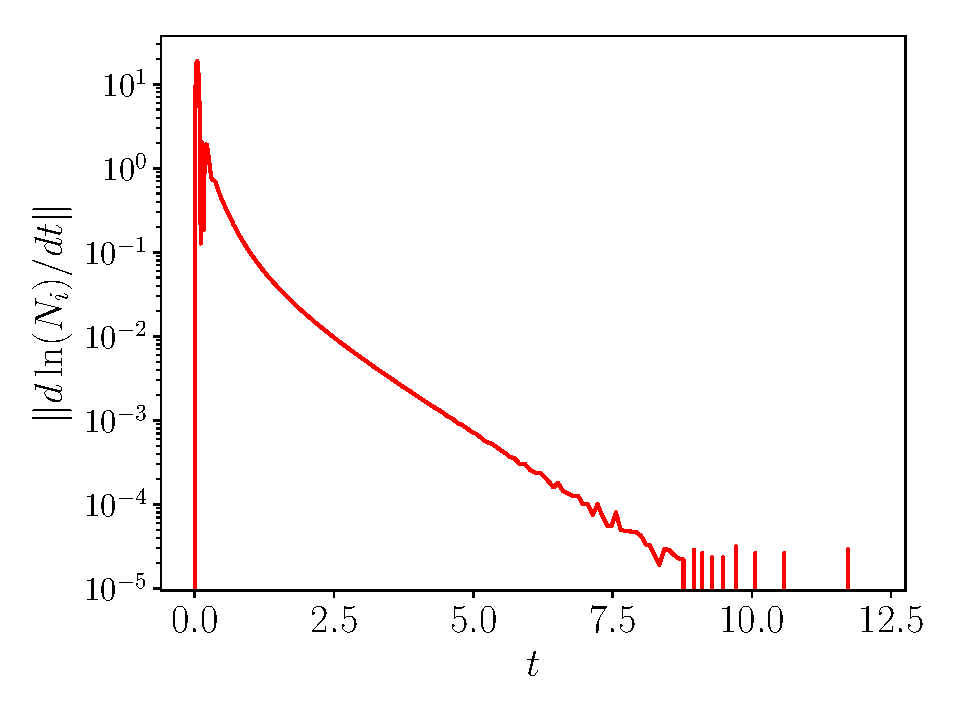
\includegraphics[width=0.6\linewidth]{figures/Typical_time_evolution/Typical_time_evolution_log_derivative_low_threshold.pdf}
% \caption{Typical convergence to judge equilibrium, we see the simulation stops at $\epsilon_{\text{conv}}=10^{-5}$}
% \end{figure}
% \subsection{Allowed parameters: syntrophy range}
% \begin{figure}[h!]
% \centering
% 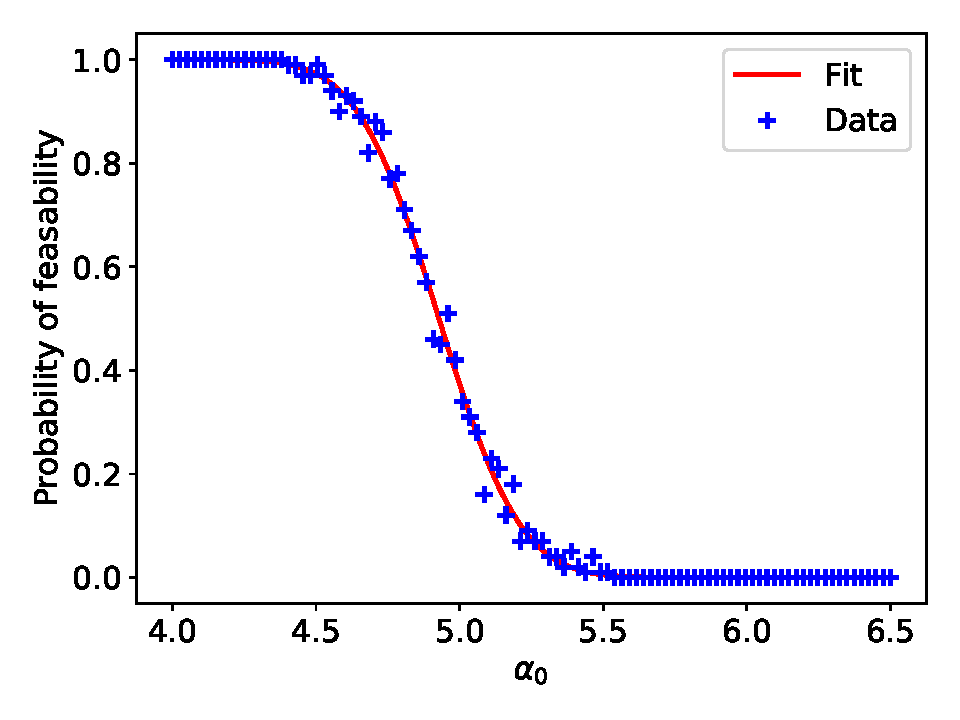
\includegraphics[scale=0.7]{figures/alpha0_probability_of_feasability}
% \caption{Typical shape of the probability of feasability for every metaparameter fixed except varying $\alpha_0$. We see that the probability of drawing a feasible system decreases sharply as $\alpha_0$ increases. A typical sigmoidal curve (here an erf function) fits the numerical data quite well.}
% \end{figure}

% \subsection{Studying the impact of the food network structure}
% \subsection{Studying the impact of syntrophy}
% We run a bunch of simulations with the following metaparameters. We made sure that these are compatible with the bounds on $\alpha_0$ Eqs.\eqref{eq: alpha bounds}.
%
% % Please add the following required packages to your document preamble:
% % \usepackage{graphicx}
% \begin{table}[h!]
% \centering
% \begin{tabular}{c|c|c|c|c|c}
% $\gamma_0$ & $\sigma_0$ & $\alpha_0$ & $R_0$ & $S_0$ & $l_0$ \\ \hline
% 1          & 1          & 0          & 300   & 1     & 11091 \\
%          & 0.75       & 0          &       &       &       \\
%          &            & 0.5        &       &       &       \\
%          & 0.5        & 0          &       &       &       \\
%          &            & 0.5        &       &       &       \\
%          &            & 1          &       &       &       \\
%          & 0.25       & 0          &       &       &       \\
%          &            & 0.5        &       &       &       \\
%          &            & 1          &       &       &       \\
%          &            & 1.5        &       &       &
% \end{tabular}
% \caption{Metaparameters used for the simulations.} \label{eq: table metaparameters used}
% \end{table}

\subsection{LRI regime -- Outcome of the Monte Carlo algorithm}
Methods \ref{section: methods LRI MC solver} explains how we designed an algorithm whose goal is to find the shape of the syntrophy matrix $A$ that should bring us closer to a dynamically stable regime for a given consumption matrix $G$. It works by minimizing an energy $E(A,G)$ given by Eq.\eqref{eq: dynamical stability methods LRI MC solver energy definition} and should, for a given $G$, yield an $A$ matrix with the following properties:
\begin{itemize}
\item Each diagonal element of $AG$ is minimized. Note that $(AG)_{\mu\mu}=\sum_{i=1}^{N_S} A_{\mu i} G_{i\mu}$ corresponds to the number of species that both consume and release resource $\mu$.
\item Outside of the diagonal, we should have $\frac{\alpha_0}{\gamma_0 R_0} AG \approx  G^T G$. A direct ecological interpretation is more difficult to draw. For a couple of different resources $(\mu,\nu)$,  $(AG)_{\mu\nu}=\sum_{i=1}^{N_S} A_{\mu i} G_{i\nu}$ is the number of species that both consume resource $\nu$ and release resource $\mu$ and $(G^TG)_{\mu\nu}=\sum_{i=1}^{N_S} G_{i\mu}G_{i\nu}$ is the number of consumers that eat both $\nu$ and $\mu$.
\end{itemize}
So intuitively the LRI MC algorithm should give us a syntrophy matrix that both limits intraspecific syntrophy and such that for every couple of different resources $(\mu, \nu)$, the number of consumers that eat both $\mu$ and $\nu$ is proportional to the number of consumers that eat $\mu$ and release $\nu$. The proportionality constant, which is the same for all $(\mu, \nu)$ is equal to the ratio of the syntrophy and consumption interactions.
 Since the connectance is and the dimensions of $A$ are fixed, the number of links of $A$ is already decided and the algorithm simply decides the optimal cells to put them in. Figure \ref{fig: dynamical stability results typical shape of consumption syntrophy LRI algorithm} shows that typically the algorithm will put links in a cell $(\mu,i)$ if $(i, \mu)$ is zero, meaning that not only intraspecific syntrophy tries to be avoided but also species that consume a lot of resources will tend to release few of them and vice-versa.
\begin{figure}
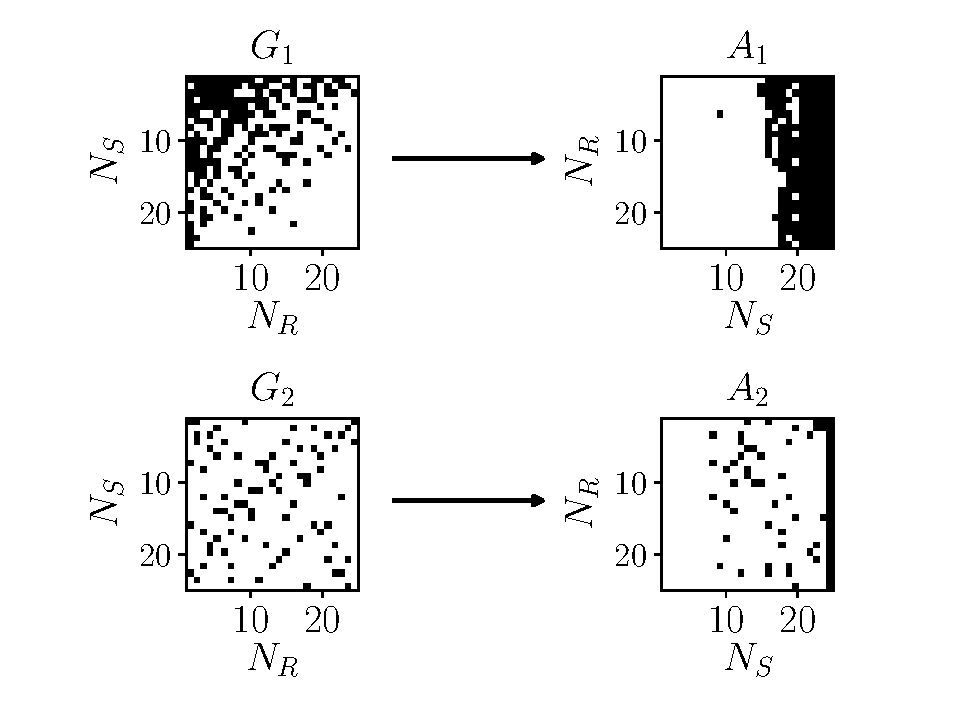
\includegraphics{typical_optimal_LRI_matrix}
\caption{Typical shape of the consumption $G_i$ and syntrophy $A_i$ matrices. The white cells symbolize a zero matrix element and the black cells, a one. $A_i$ here is the outcome of the LRI MC algorithm described in Methods \ref{section: methods LRI MC solver}. The first row has a consumption matrix with $\eta_1=0.6$ and $\kappa_1=0.32$, the LRI MC solver gives rise to a syntrophy matrix with same connectance and ecological overlap $\approx 0.85$. The second row has $G_2$ with $\eta_2=0.1$ and $\kappa_2=0.13$ and the corresponding syntrophy matrix $A_2$ has ecological overlap $\sim 0.42$. We observe that under this optimisation, species that consume few resources end up releasing many and the other way around.}\label{fig: dynamical stability results typical shape of consumption syntrophy LRI algorithm}
\end{figure}
Figure \ref{fig: dynamical stability optimal LRI requirements met} shows that indeed we obtain for a given $G$ matrix a syntrophy matrix $A$ such that the two requirements above are best satisfied. Note that the algorithm works better for matrices with a low connectance.
\begin{figure}
  \begin{minipage}[c]{0.67\textwidth}
    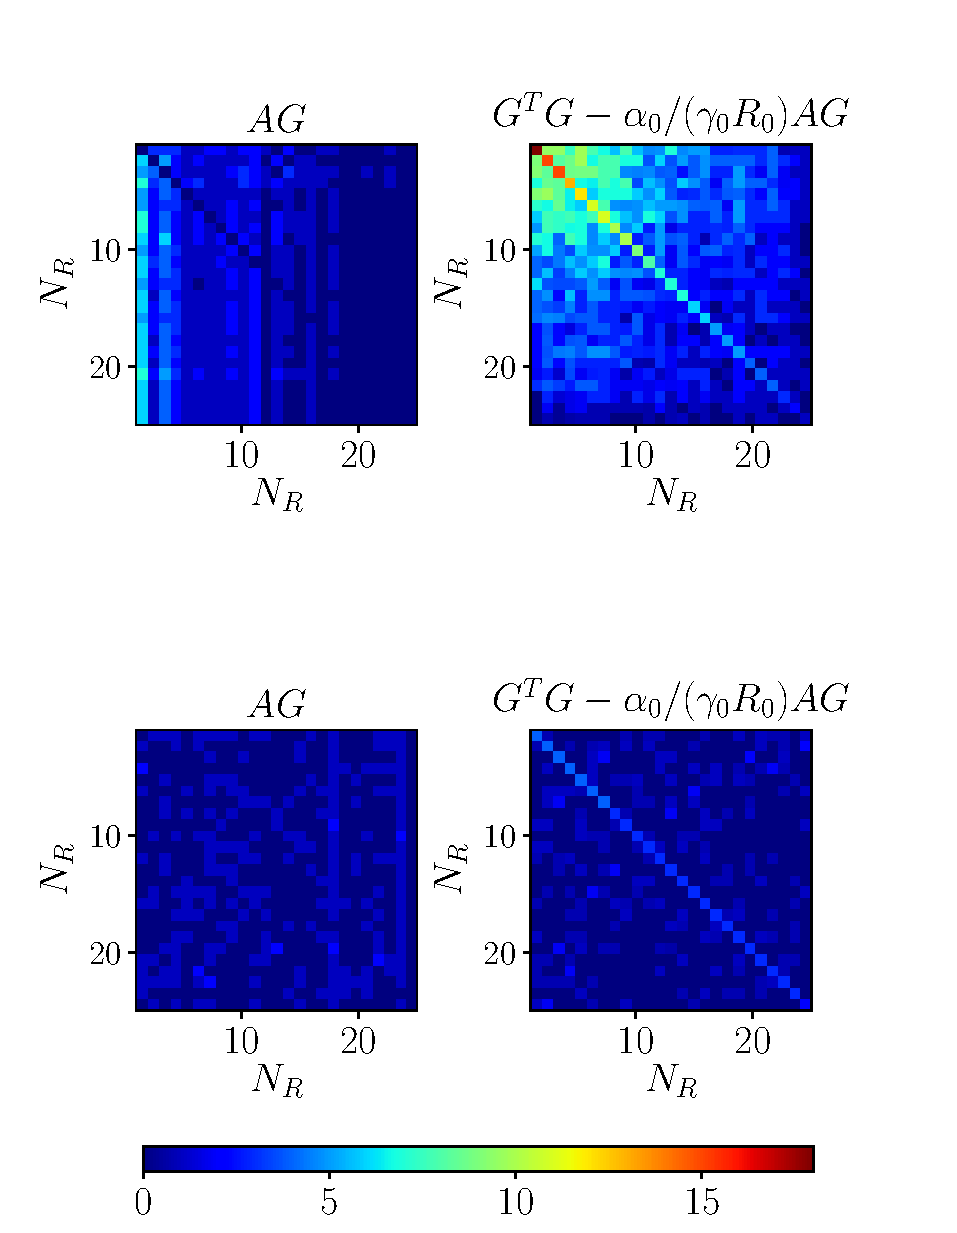
\includegraphics[width=\textwidth]{optimal_LRI_requirements}
  \end{minipage}\hfill
  \begin{minipage}[c]{0.3\textwidth}
    \caption{Plotting of $AG$ and $G^TG-\alpha_0/(\gamma_0R_0) AG$. The $A$ and $G$ matrices of the first and second rows correspond to the respective $A$ and $G$ of Figure \ref{fig: dynamical stability results typical shape of consumption syntrophy LRI algorithm}. As expected, we obtain an $A$ such that intraspecific coprophagy is limited (the diagonal of $AG$ is roughly zero) and, outside the diagonal, $G^TG-\alpha_0/(\gamma_0R_0) AG \approx 0$. Both relations are better satisfied for consumption (and hence syntrophy) matrices with a low connectance.}\label{fig: dynamical stability optimal LRI requirements met}
  \end{minipage}
\end{figure}
It is worth noticing that this procedure produces highly nested syntrophy matrices (Fig.\ref{fig: dynamical stability results nestedness LRI outcome}) where only a few species produce most of the syntrophic flow. The obtained matrices have an even larger nestedness if we increase the number of resources.
\begin{figure}
\captionsetup[subfigure]{captionskip = -180pt, margin = 42pt}
\hspace{-0.1\linewidth}
\subfloat[]{\includegraphics[width=0.6\linewidth]{{structure_alpha_matrix_NR25_NS25_with_nestedness}.pdf}}
\subfloat[]{\includegraphics[width=0.6\linewidth]{{structure_alpha_matrix_NR25_N25_with_connectance}.pdf}}

\hspace{-0.1\linewidth}
\subfloat[]{\includegraphics[width=0.6\linewidth]{{structure_alpha_matrix_NR50_NS25_with_nestedness}.pdf}}
\subfloat[]{\includegraphics[width=0.6\linewidth]{{structure_alpha_matrix_NR50_N25_with_connectance}.pdf}}
\caption{Properties of the syntrophy matrix against the consumption matrix. (a)-(c) Ecological overlap of $A$ as a function of the ecological overlap of $G$ for $N_S=25$ and $N_R=25$ (a) or $N_R=50$ (c). (b)-(d) Ecological overlap of $A$ as a function of the connectance of $G$ for $N_S=25$ and $N_R=25$ (b) or $N_R=50$ (d). The nestedness of the ``intraspecific syntrophy restricted'' is also plotted as a matter of comparison. As $\eta_G$ or $\kappa_G$ increase, the two results will without surprise give matrices with similar properties. \textbf{Explain this?}}
\label{fig: dynamical stability results nestedness LRI outcome}
\end{figure}

\FloatBarrier
\subsection{Fully dynamically stable region}
The same way we studied the fully feasible volume $\mathcal{F}_{1}^{G,A}(\alpha_0)$, we investigate now the behaviour of its special subset, the locally fully dynamically stable region $\mathcal{D}^{G,A}_{L,1}\left(\alpha_0\right)$. A formal definition of $\mathcal{D}^{G,A}_{L,1}\left(\alpha_0\right)$ is provided in Methods \ref{sec: dynamical stability methods locally dynamically stable region}. Intuitively, $\mathcal{D}^{G,A}_{L,1}\left(\alpha_0\right)$ corresponds to the set of all metaparameters $m \in \mathcal{M}$ such that $\mathcal{A}(m, G, A)$ is a feasible, locally dynamically stable system with probability 1. Since we require $\mathcal{A}(m, G, A)$ to be feasible, it is clear that $\mathcal{D}^{G,A}_{L,1}\left(\alpha_0\right)$ is indeed a subset of $\mathcal{F}^{G,A}_1\left(\alpha_0\right)$.

Figure \ref{fig: dynamical stability results local dynamical stability region for different matrices} shows
that $\mathcal{D}_{L,1}^{G,A}\left(\alpha_0\right)$ is geometrically more complex than $\mathcal{F}_{1}^{G,A}\left(\alpha_0\right)$ (which is after all not suprising, the question of dynamical feasibility is harder than the one of feasibility!). It may sometimes have holes, even without syntrophy, and sometimes not, even for matrices that are topologically very close. Compare for instance Fig.\ref{fig: lds region results Nest 0.35 Conn 0.2208} with Fig.\ref{fig: lds region results Nest 0.35 Conn 0.272}, these two networks have the same ecological overlap, but even though their connectance is very similar, their fully locally dynamically stable regions have a very different shape: one of them can sustain only a tiny bit of syntrophy before becoming dynamically unstable (Fig.\ref{fig: lds region results Nest 0.35 Conn 0.2208}) while the second can endure basically any feasible syntrophic interaction (Fig.\ref{fig: lds region results Nest 0.35 Conn 0.272}). A general trend is hence harder to find but it seems that points with a larger $\gamma_0$ are in general more dynamically stable (more on this below).
\begin{figure}
\captionsetup[subfigure]{captionskip = -185pt, margin = 52pt}
\vspace{-96pt}
\hspace{-0.1\linewidth}
\subfloat[\label{fig: lds region results Nest 0.35 Conn 0.2208}]{\includegraphics[width=1.2\linewidth]{{local_dynamical_stability_wt_wc_region_NR25_NS25_Nest0.35_Conn0.2208}.pdf}}

\vspace{-68pt}
\hspace{-0.1\linewidth}
\subfloat[]{\includegraphics[width=1.2\linewidth]{{local_dynamical_stability_wt_wc_region_NR25_NS25_Nest0.35_Conn0.3216}.pdf}}

\vspace{-68pt}
\hspace{-0.1\linewidth}
\subfloat[\label{fig: lds region results Nest 0.35 Conn 0.272}]{\includegraphics[width=1.2\linewidth]{{local_dynamical_stability_wt_region_NR25_NS25_Nest0.35_Conn0.272}.pdf}}

\caption{Locally fully dynamically stable region $\mathcal{D}_{L,1}^{G,A}$ as a function of syntrophy for different matrices $G$. The white zone corresponds to points that are never fully locally dynamically stable. The colour of a given point tells until which syntrophy that point is fully locally dynamically stable, \eg
a green point is fully locally dynamically stable for $0 \leq \alpha_0 \leq \num{6.5e-3}$. Row (a) corresponds to $G$ with $\eta_G = 0.35$ and $\kappa_G = 0.23$, (b) has $\eta_G=0.35$ and $\kappa_G=0.33$ and (c) $\eta_G=0.35$ and $\kappa_G=0.27$. Even at fixed ecological overlap, different connectances of $G$ give rise to completely different systems in terms of local dynamical stability.}\label{fig: dynamical stability results local dynamical stability region for different matrices}
\end{figure}
We required that a system had to be feasible in order to be dynamically stable, which is the mathematical equivalent of $\mathcal{D}_{L,1}^{G,A}(\alpha_0) \subset \mathcal{F}_1^{G,A}\left(\alpha_0\right)$, \ie local dynamical stability implies feasibility. We may also ask the reverse question, does feasibility imply local dynamical stability?
The answer to this is, again, unsurpisingly, ``it depends on the matrix'', as shows Figure \ref{fig: dynamical stability results local dynamical stability region for different matrices}. For instance, for $G$ with $\kappa_G=0.13$ and $\eta_G=0.1$, we have $\text{Vol}\left(\mathcal{D}_{L,1}^{G,A}(\alpha_0)\right) < \text{Vol}\left(\mathcal{F}_{L,1}^{G,A}(\alpha_0)\right) \forall \alpha_0$, which means that for this consumption matrix feasibility does not imply stability. The fully connected case gives a larger dynamically stable volume than the regime without intraspecific syntrophy which is itself better than the LRI regime. This hints that the LRI regime, despite what it was designed for, apparently does not give better results than other structures of $A$.
 On the contrary, for $G$ with $\kappa_G=0.32$ and $\eta_G=0.6$, both volumes are equal at every syntrophy that is feasible, for the three structures of $A$ considered, which shows that for this specific matrix, feasibility implies local dynamical stability.
\begin{figure}
\captionsetup[subfigure]{captionskip = -230pt, margin = 50pt}
\vspace{-96pt}
\hspace{-0.1\linewidth}
\subfloat[]{\includegraphics[width=1.2\linewidth]{{feasibility_vs_lds_NR25_NS25_Nest0.1_Conn0.1296}.pdf}}

\hspace{-0.1\linewidth}
\subfloat[]{\includegraphics[width=1.2\linewidth]{{feasibility_vs_lds_NR25_NS25_Nest0.6_Conn0.3168}.pdf}}

\caption{Ratio of the size of the fully dynamically stable volume and the fully feasible volume for two consumption matrices $G$ (a) with $\eta_G=0.1$ and $\kappa_G=0.13$, (b) with $\eta_G=0.6$ and $\kappa_G=0.32$. We observe different behaviours for different matrices: for (a) feasibility does not imply local dynamical stability even without syntrophy (it is barely feasible but the ratio is a bit below one for $\alpha_0=0$). On the other hand, for (b) feasibility implies local dynamical stability, indeed both regions have the same volume and since $\mathcal{D}_{L,1}^{G,A}(\alpha_0) \subset \mathcal{F}^{G,A}_1(\alpha_0)$, we conclude that both are equal.}
\end{figure}
A good way to measure how systems react to syntrophy is to compute the \important{critical locally dynamically stable syntrophy} $\alpha_0^D(G,A)$ (see Methods \ref{sec: methods dynamical stability}). An easy way this can be done is by getting some points of the volume of $\mathcal{D}_{L,1}^{G,A}\left(\alpha_0\right)$ curve and finding its intercept to zero. Figure \ref{fig: dynamical stability results typical shrinkage of dynamical volume} shows the typical shrinkage of the fully locally dynamically stable volume.
\begin{figure}
\centering
\includegraphics[width=0.6\linewidth]{{size_of_dynamical_volume_NR25_NS25_Nest0.5_Conn0.416}.pdf}
\caption{Evolution of the volume of $\mathcal{D}_{L,1}^{G,A}\left(\alpha_0\right)$ with $\alpha_0$ for a consumption matrix $G$ with $\eta_G=0.5$ and $\kappa_G=0.42$. The size of the fully locally dynamically feasible region shrinks as syntrophy increases. A linear fit is performed on the last four points to determine $\alpha_0^D(G,A)$ (see Fig.\ref{fig: dynamical stability results critical dynamical syntrophy}), the point where this curves reaches zero.}
\label{fig: dynamical stability results typical shrinkage of dynamical volume}
\end{figure}
To find $\alpha_0^D(G,A)$ for each $G$, we fit with a linear function the last four points of the curve corresponding to Fig.\ref{fig: dynamical stability results typical shrinkage of dynamical volume} and find its intercept to zero $\alpha_0^D(G,A)$. Figure \ref{fig: dynamical stability results critical dynamical syntrophy} shows a very interesting and clear behaviour\footnote{Those results have to be taken with a grain of salt because we did not check whether $\alpha_0^D(G,A)$ was feasible, \ie the actual critical locally dynamically stable syntrophy is the minimum between the value measured in Fig.\ref{fig: dynamical stability results critical dynamical syntrophy} and the largest feasible $\alpha_0$ for that couple $(G,A)$.}: for a given connectance of the consumption matrix, systems that can sustain the largest syntrophy have a small ecological overlap. And for a given ecological overlap, systems with a larger connectance will stay stable longer under the action of syntrophy. In the end, optimal systems have a small ecological overlap and a large connectance: many resources are eaten by the consumers, but they do not share them.



\begin{figure}
\captionsetup[subfigure]{captionskip = -185pt, margin = 52pt}
\vspace{-84pt}
\hspace{-0.1\linewidth}
\subfloat[]{\includegraphics[width=0.6\linewidth]{{largest_eigenvalue_NR25_NS25_critical_alpha0_fixed_connectance_random_structure}.pdf}}
\subfloat[]{\includegraphics[width=0.6\linewidth]{{largest_eigenvalue_NR25_NS25_critical_alpha0_fixed_nestedness_random_structure}.pdf}}

\vspace{-12pt}
\hspace{-0.1\linewidth}
\subfloat[]{\includegraphics[width=0.6\linewidth]{{largest_eigenvalue_NR25_NS25_critical_alpha0_fixed_connectance_no_release_when_eat}.pdf}}
\subfloat[]{\includegraphics[width=0.6\linewidth]{{largest_eigenvalue_NR25_NS25_critical_alpha0_fixed_nestedness_no_release_when_eat}.pdf}}

\vspace{-12pt}
\hspace{-0.1\linewidth}
\subfloat[]{\includegraphics[width=0.6\linewidth]{{largest_eigenvalue_NR25_NS25_critical_alpha0_fixed_connectance_optimal_matrix}.pdf}}
\subfloat[]{\includegraphics[width=0.6\linewidth]{{largest_eigenvalue_NR25_NS25_critical_alpha0_fixed_nestedness_optimal_matrix}.pdf}}
\vspace{-12pt}
\caption{Critical syntrophy $\alpha_0^D$, defined as the smallest syntrophy for which we can still find metaparameters that will give rise to fully dynamically stable systems. How $\alpha_0^D$ is estimated is explained in the main text. Errors on $\alpha_0^D$ are not plotted but are at most around $10\%$. (a)(c)(e) Evolution of $\alpha_0^D$ with ecological overlap $\eta$ at different connectance. (b)(d)(f) Evolution of $\alpha_0^D$ with connectance $\kappa$ for different ecological overlap. We observe a strong trend: for a given connectance, $\alpha_0^D$ decreases as ecological overlap increases. Also, for a given ecological overlap, $\alpha_0^D$ increases as connectance is increased.}\label{fig: dynamical stability results critical dynamical syntrophy}
\end{figure}
Finally, one can take a look at the \important{common fully locally dynamically stable region}, which is the intersection of the $\mathcal{D}_{L,1}^{G,A}(\alpha_0) \forall (G,A) \in S_M$ (Figure \ref{fig: dynamical stability results common fully dynamically stable volume}). Because of the fractured and heterogenous nature of each $\mathcal{D}_{L,1}^{G,A}(\alpha_0)$, we observe a very fractured and small common fully locally dynamically stable region, which is the same for all structures of $A$ considered. It has a non-zero volume for $\alpha_0=0$, but for the next point investigated $\alpha_0=\num{1.3e-3}$, no point is fully locally dynamically stable for every matrix considered, which means that the critical common syntrophy is smaller than this.
\begin{figure}
\vspace{-84pt}
\hspace{-0.1\linewidth}
\subfloat[]{\includegraphics[width=0.6\linewidth]{{common_local_dynamical_stability_volume_NR25_NS25_varying_syntrophy_random_structure}.pdf}}
\subfloat[]{\includegraphics[width=0.6\linewidth]{{common_local_dynamical_stability_volume_NR25_NS25_varying_syntrophy_no_release_when_eat}.pdf}}

\centering
\subfloat[]{\includegraphics[width=0.6\linewidth]{{common_local_dynamical_stability_volume_NR25_NS25_varying_syntrophy_optimal_matrix}.pdf}}
\caption{Common full local dynamical stability volume for different $A$ structures: (a) fully connected, (b) no intraspecific syntrophy and (c) LRI algorithm. The points coloured in dark red give rise to locally dynamically stable systems with probability 1 for \important{all the matrices considered}. Very few spots verify this property when there is no syntrophic interaction, and no point gives rise to a fully dynamically stable system for $\alpha_0 = \num{1.3e-3}$. This is independent of the structure of $A$ that we chose. The white points never give rise to fully dynamically stable systems.}\label{fig: dynamical stability results common fully dynamically stable volume}
\end{figure}

\FloatBarrier
\subsection{Largest eigenvalue of the jacobian}
Equation \eqref{eq: dynamical stability methods fully connected metaparameters} from Methods \ref{sec: methods dynamical stability fully connected zero variance} gives a relationship that the metaparameters should approximately follow in order to give rise to locally dynamically stable systems. Although strictly speaking it is only valid for the case where both $G$ and $A$ are fully connected, we expect it to work as well when $G$ and $A$ are \important{not too far away} from the fully connected case. It tells us that in order to get more local dynamically stable systems you should:
\begin{itemize}
  \item decrease $N_S$, $l_0$ \textbf{WEIRD RESULT: would expect that increasing l0 would make systems more dynamically stable (observed in simulations I think)} or $\alpha_0$,
  \item if $\alpha_0 - \gamma_0 R_0 < 0$, increase $N _R$, $\sigma_0$ and $\gamma_0$,
  \item be careful in how you handle $S_0$: increasing $S_0$ reduces the $l_0^2/S_0$ term but increases the $N_S^2 \alpha_0^2 S_0$ term. It is very easy to show (Appendix \ref{sec: appendix how to handle S0}) that if $S_0 > l_0/(N_S \alpha_0)$ it should be decreased, and otherwise it should be increased until it reaches $l_0/(N_S \alpha_0)$.
\end{itemize}

Combining these with the feasibility conditions Eq.\eqref{eq: fully feasible volume} we expect that -- for all other metaparameters fixed -- systems get more and more locally dynamically stable as $\gamma_0$ is increased and $S_0$ is the largest possible. In short, points at the upper border of $\mathcal{D}^{G,A}_{L,1}$ should have a lower and lower $\real{\lambda_1}$ as $\gamma_0$ increases. Figure \ref{fig: local dynamical stability results largest eigenvalue} shows that indeed this trend is followed.
\begin{figure}
\vspace{-72pt}
\hspace{-0.0\linewidth}
\subfloat[]{\includegraphics[width=\linewidth]{{largest_eigenvalue_wt_NR25_NS25_Nest0.1_Conn0.1296_alpha0=0.0}.pdf}}

\vspace{-26pt}
\hspace{-0.0\linewidth}
\subfloat[]{\includegraphics[width=\linewidth]{{largest_eigenvalue_wt_NR25_NS25_Nest0.1_Conn0.1296_alpha0=0.0039}.pdf}}

\vspace{-26pt}
\hspace{-0.0\linewidth}
\subfloat[]{\includegraphics[width=\linewidth]{{largest_eigenvalue_wt_NR25_NS25_Nest0.1_Conn0.1296_alpha0=0.0078}.pdf}}
\caption{Largest real eigenvalue $\text{Re}(\lambda_1)$ averaged over 300 realisations for each $(\gamma_0, S_0)$ points for the consumption matrix $G$ with consumers overlap $\eta_G = 0.1$ and connectance $\kappa_G=0.13$. The white points correspond to not fully dynamically stable systems. Each row corresponds to a different syntrophy value (a) $\alpha_0 = 0$ (no syntrophic interaction), (b) $\alpha_0 = \num{3.9e-3}$ and (c) $\alpha_0 = \num{7.8e-3}$. The first column corresponds to the regime where $A$ is fully connected, the second where $A$ forbids intraspecific syntrophy and the third is the outcome of the MC algorithm. As syntrophy increases, the size of the fully dynamically stable region decreases. Furthermore, the boundary points close to the $\gamma_0 \sim S_0^{-1}$ curve are the most stable in every situation.}\label{fig: local dynamical stability results largest eigenvalue}
\end{figure}
This tells us that if we keep the consumption flux $N_S \gamma_0 S_0$ constant, increasing $\gamma_0$ (and hence decreasing $S_0$) will give rise to more stable systems. Notice that contrarily to the prediction made above, increasing $\alpha_0$ does not decrease stability but increases the maximal $\abs{\real{\lambda_1}}$ observed as shows Fig.\ref{fig: dynamical stability results typical maximal eigenvalue observed varying syntrophy}. This is coupled with the shrinkage of the fully locally dynamically stable volume seen on Fig.\ref{fig: dynamical stability results shrinkage of DL1G varying syntrophy}. This means that overall increasing syntrophy makes the system \important{more stable} but at \important{fewer points}. This hints that systems in a high syntrophic regime, where consumers produce a lot of resources, should be very fine-tuned and occur for very specific consumption strength and average abundance of consumers.
\begin{figure}
\hspace{-0.1\linewidth}
\captionsetup[subfigure]{captionskip = -210pt, margin = 26pt}
\subfloat[\label{fig: dynamical stability results typical maximal eigenvalue observed varying syntrophy}]{\includegraphics[width=0.6\linewidth]{{largest_eigenvalue_varying_syntrophy_NR25_NS25_Nest0.3_Conn0.2272}.pdf}}
\subfloat[\label{fig: dynamical stability results shrinkage of DL1G varying syntrophy}]{\includegraphics[width=0.6\linewidth]{{size_local_dynamical_stability_region_NR25_NS25_Nest0.3_Conn0.2272}.pdf}}
\caption{For a consumption matrix $G$ with $\eta_G=0.3$ and $\kappa_G=0.23$. (a) Evolution of the maximal $\abs{\av{\real{\lambda_1}}}$ observed in the $(\gamma_0,S_0) \in [0,1]^2$ region. The maximal eigenvalue increases in magnitude, making the system more dynamically stable, as syntrophy increases. That trend is true for all matrices we considered. (b) Volume of $\mathcal{D}^G_{L,1}(\alpha_0)$. As syntrophy increases, fewer and fewer points become fully dynamically stable. For both figures, the different lines show the different stand for the different structure of the syntrophy matrix that we considered.}\label{fig: results dynamical stability maximum eigenvalue observed vs size of dynamical region 25x25}
\end{figure}

\FloatBarrier
\subsection{The influence of the matrix dimension}
As said above, because of Eq.\eqref{eq: dynamical stability methods fully connected metaparameters}, we expect stability to increase when the number of resources is increased for a fixed number of consumers. The following subsection shows what happens when the number of resources is doubled $N_R=25 \rightarrow N_R=50$ and every other metaparameter, as well as the number of consumers, keeps the same value as before.

Figure \ref{fig: dynamical stability results typical lds region NR=50 NS=25} shows that the effect of adding resources can be quite dramatic on the stability of the system. For that specific matrix for instance, adding resources allowed for a way larger $\mathcal{D}^{G,A}_{L,1}\left(\alpha_0\right)$ at each $\alpha_0$. It even allows full dynamical stability in the feasibility region for larger syntrophic interactions than before.
\begin{figure}[h]
\subfloat[]{\includegraphics[width=\linewidth]{{local_dynamical_stability_region_NR25_NS25_Nest0.45_Conn0.3168}.pdf}}

\subfloat[]{\includegraphics[width=\linewidth]{{local_dynamical_stability_region_NR50_NS25_Nest0.45_Conn0.3328}.pdf}}
\caption{Fully dynamically stable region $\mathcal{D}^{G,A}_{L,1}$ with the three different structures of $A$ considered: fully connected (left), no intraspecific syntrophy (middle) and LRI matrix (right). The two matrices have the same ecological overlap and connectance, only the number of resources changes. (a) $G$ has $N_R=25$, $N_S=25$ and $\kappa_G=0.32$ and $\eta_G=0.45$. (b) $G$ has $N_R=50$, $N_S=25$ and $\kappa_G=0.33$ and $\eta_G=0.45$. The fact that more points can sustain an increased syntrophy is a trend for most of the matrices of the set. \textbf{still check this: the others are more less the same or a tad less}.} \label{fig: dynamical stability results typical lds region NR=50 NS=25}
\end{figure}
Even though more syntrophy can be sustained, it seems that the volume of $\mathcal{D}_{L,1}^{G,A}(\alpha_0)$ is smaller at $N_R=50$ than at $N_R=25$ (compare for  instance Fig.\ref{fig: dynamical stability results shrinkage of DL1G varying syntrophy NR=50} with Fig.\ref{fig: dynamical stability results shrinkage of DL1G varying syntrophy}). This is compensated by the fact that way larger eigenvalues are observed at $N_R=50$: although there are (a bit) fewer equilibrium points, these are more stable (compare Fig.\ref{fig: dynamical stability results typical maximal eigenvalue observed varying syntrophy NR=50} and Fig.\ref{fig: dynamical stability results typical maximal eigenvalue observed varying syntrophy}). This is a trend that we believe holds for all the matrices considered but a more thorough investigation should be conducted before claiming those results to be absolutely true.
\begin{figure}
\hspace{-0.1\linewidth}
\captionsetup[subfigure]{captionskip = -210pt, margin = 26pt}
\subfloat[\label{fig: dynamical stability results typical maximal eigenvalue observed varying syntrophy NR=50}]{\includegraphics[width=0.6\linewidth]{{largest_eigenvalue_varying_syntrophy_NR50_NS25_Nest0.3_Conn0.2296}.pdf}}
\subfloat[\label{fig: dynamical stability results shrinkage of DL1G varying syntrophy NR=50}]{\includegraphics[width=0.6\linewidth]{{size_local_dynamical_stability_region_NR50_NS25_Nest0.3_Conn0.2296}.pdf}}
\caption{To be compared with Fig.\ref{fig: results dynamical stability maximum eigenvalue observed vs size of dynamical region 25x25}. The consumption matrix $G$ considered here has $\eta_G=0.3$ and $\kappa_G=0.23$. (a) Maximal average $\abs{\real{\lambda_1}}$ observed in the unit square. (b) Percentage of the unit square occupied by the fully dynamically stable region of $G$ as a function of syntrophy. The matrix considered has almost equal properties to the one in Fig.\ref{fig: results dynamical stability maximum eigenvalue observed vs size of dynamical region 25x25}, with the only difference that $N_R=50$ here. Even though the size of $\mathcal{D}_{L,1}^{G,A}$ is smaller, the eigenvalues are larger in magnitude.}
\end{figure}

% \begin{figure}
% \vspace{-72pt}
% \hspace{-0.0\linewidth}
% \subfloat[]{\includegraphics[width=\linewidth]{{largest_eigenvalue_wt_NR50_NS25_Nest0.1_Conn0.0832_alpha0=0.0}.pdf}}
%
% \vspace{-26pt}
% \hspace{-0.0\linewidth}
% \subfloat[]{\includegraphics[width=\linewidth]{{largest_eigenvalue_wt_NR50_NS25_Nest0.1_Conn0.0832_alpha0=0.0013}.pdf}}
%
% \vspace{-26pt}
% \hspace{-0.0\linewidth}
% \subfloat[]{\includegraphics[width=\linewidth]{{largest_eigenvalue_wt_NR50_NS25_Nest0.1_Conn0.0832_alpha0=0.0039}.pdf}}
% \caption{To be compared with \ref{fig: local dynamical stability results largest eigenvalue} \textbf{Is it really fair? No comparison because connectance is overall quite different and we saw that changing connectance can have quite a dramatic effect}, the zone is smaller but more stable (by a lot) can we really say this?.}\label{fig: dynamical stability results largest eigenvalue NR=50 NS=25}
% \end{figure}

Since matrices are individually more locally dynamically stable, the \important{common locally dynamically stable} region is larger with $N_R=50$ resources than with $N_R=25$. The difference between Figure \ref{fig: dynamical stability results common fully dynamically stable volume} and Figure \ref{fig: dynamical stability results common lds volume NR=50 NS=25} is very striking: when the number of resources is increased not only is $\mathcal{D}_{L,1}^{S_M}\left(\alpha_0\right)$ larger, it also can overall bear a larger syntrophy. Remember that for $N_R=25$, the critical common syntrophy was between $0$ and $\num{1.3e-3}$, and for $N_R=50$, it is way larger, between $\num{3.9e-3}$ and $\num{5.2e-3}$. \textbf{Is there anything more to add? I have some plots but I am not sure if they are the most relevant}

\begin{figure}
\vspace{-84pt}
\hspace{-0.1\linewidth}
\subfloat[]{\includegraphics[width=0.6\linewidth]{{common_local_dynamical_stability_volume_NR50_NS25_varying_syntrophy_random_structure}.pdf}}
\subfloat[]{\includegraphics[width=0.6\linewidth]{{common_local_dynamical_stability_volume_NR50_NS25_varying_syntrophy_no_release_when_eat}.pdf}}

\centering
\subfloat[]{\includegraphics[width=0.6\linewidth]{{common_local_dynamical_stability_volume_NR50_NS25_varying_syntrophy_optimal_matrix}.pdf}}
\caption{Common fully dynamically stable volume. It is larger with a larger number of resources -> even though individually it is not always better, it is better for the worse matrices (since the common volume can handle more syntrophy)}\label{fig: dynamical stability results common lds volume NR=50 NS=25}
\end{figure}









\end{document}
